%نام و نام خانوادگی:
%شماره دانشجویی: 
\مسئله{منظور از باگ در یک وب سایت یا موبایل اپلیکیشن چیست؟ با استفاده از مثال از سایت‌ها یا اپلیکیشن‌های مختلف 5 نمونه باگ بنویسید.\\}
 


\پاسخ{

در تست نرم‌افزار اصطلاحات متنوعی برای خطا استفاده می‌شود که در زبان فارسی همه به خطا یا باگ ترجمه می‌شوند. هنوز بر سر تعریف دقیق این اصطلاحات اختلاف نظر است و ممکن است موقع استفاده از آن‌ها شنونده آنچه که منظور شماست را متوجه نشود. این اصطلاحات را در ادامه به اختصار توضیح می‌دهیم. \cite{360logica}


\begin{itemize}
	\item خطا (Defect) :
	تفاوت بین نتایج مورد انتظار و نتایج واقعی در هنگام تست است که در واقع انحراف از نیاز مشتری است.
	
	\item خطا (Error) :
	خطا یک اشتباه، تصور اشتباه یا سوء تفاهم از سوی یک توسعه دهنده نرم افزار است. برای مثال یک برنامه نویس ممکن است نام متغیر را به اشتباه تایپ کند.
	
	\item باگ (Bug) :
	یک باگ نتیجه اشتباه در کد است. خطایی که قبل از ارسال محصول به مشتری، در محیط توسعه یافت می شود. یک خطای برنامه نویسی که باعث می شود برنامه ضعیف کار کند، نتایج نادرست ایجاد کند یا کرش کند. یک خطا در نرم افزار یا سخت افزار که باعث اختلال در عملکرد یک برنامه می شود.
	
	\item شکست (Failure) :
	ناتوانی یک سیستم یا کامپوننت نرم افزاری در انجام موارد نیاز در چارچوب نیاز‌های عملکردی و کیفی. هنگامی که یک نقص (defect) به مشتری نهایی می رسد به آن شکست (failure) می گویند. در طول توسعه، شکست‌ها معمولاً توسط تسترها مشاهده می شوند.
	
	\item خطا (Fault) :
	نتیجه خطا (error) است. 
	
\end{itemize}

\section*{مثال‌ها}

\subsection*{مثال ۱}
\href{https://webeloperssut.com}{وبسایت رویداد وبلوپرز}.
 در شکل \ref{fig:bug1} مشاهده می‌کنیم که زمان‌سنجی که برای شمارش معکوس استفاده شده است زمانی منفی را نمایش می‌دهد. این یک باگ است و اصولا باید بجای عدد منفی زمان صفر در اینجا نمایش داده شود یا بجای زمان‌سنج، متنی با پیام «تیم‌کشی به پایان رسید.» نمایش داده شود.

\begin{figure}[H]
	\centering
	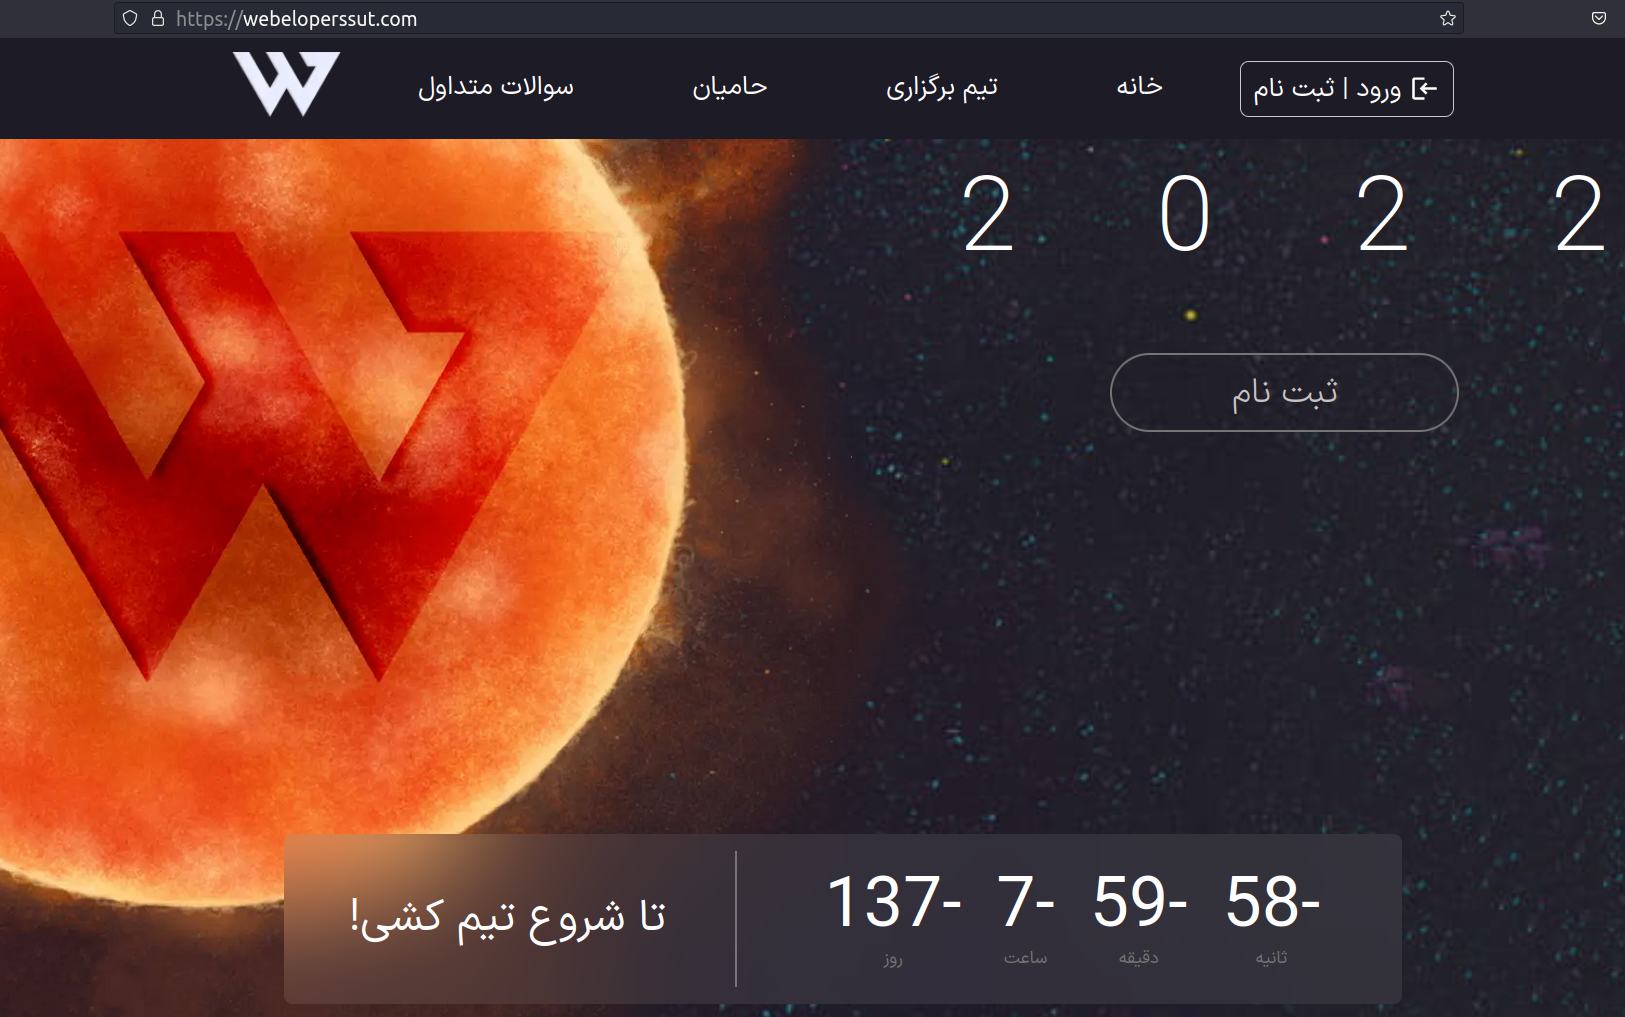
\includegraphics[width=0.7\linewidth]{figs/bug1}
	\caption[صفحه اصلی وب‌سایت رویداد وبلوپرز شریف]{صفحه اصلی وب‌سایت رویداد وبلوپرز شریف}
	\label{fig:bug1}
\end{figure}


\subsection*{مثال ۲}


در \href{ssc.ce.sharif.edu}{وب‌سایت انجمن علمی دانشکده} دکمه‌ای جهت تغییر زبان سایت وجود دارد. این دکمه در نوار بالا در دسترس می‌باشد. با کلیک بر این دکمه صفحه مجدد بارگذاری می‌شود اما تغییری صورت نمی‌گیرد.
شکل \ref{fig:bug2} تصویر وب‌سایت را در حالت زبان انگلیسی نمایش می‌دهد که هیچ تفاوتی با حالت فارسی ‌آن ندارد.
\begin{figure}[H]
	\centering
	
\includegraphics[width=0.7\linewidth]{figs/bug2}
	\caption[صفحه اصلی وب‌سایت انجمن علمی دانشکده مهندسی کامپیوتر شریف]{صفحه اصلی وب‌سایت انجمن علمی دانشکده مهندسی کامپیوتر شریف}
	\label{fig:bug2}
\end{figure}


\subsection*{مثال ۳}
\href{https://torob.com/feedback/}{فرم بازخورد وب‌سایت ترب}.
می‌دانیم که شماره تماس‌های همراه در ایران از قاعده‌ی خاصی پیروی می‌کند. شماره‌ها با ۰۹ شروع می شوند رقم سوم  می‌تواند یک (همراه اول) یا سه (ایرانسل و تالیا) یا دو (رایتل) باشد. \cite{phoneregex}

در شکل \ref{fig:bug3} مشاهده می‌شود که در فرم بازخورد وب‌سایت ترب این قاعده بررسی نمی‌شود و به همین دلیل امکان وارد کردن شماره تماس نامعتبری مانند ۰۹۰۰۰۰۰۰۰۰۰ و ثبت موفق بازخورد وجود دارد. این هم یک باگ است و هم می‌تواند یک مشکل امنیتی باشد. چرا که شخص می‌تواند با تعداد زیادی شماره تماس غیر معتبر پیام‌های بی‌معنی یا بی‌موردی را ارسال کند و موجب اسپم شدن بخش پشتیبانی ترب شود. البته باید اشاره کرد که شرکت ایرانسل جدیدا پیش‌شماره‌های ۰۹۰۰ را اضافه کرده است که در زمان نگارش مرجع ما (\cite{phoneregex}) هنوز وجود نداشته است. با این حال همچنان این فرم بدون بررسی لاگین بودن یا نبودن کاربر اجازه ثبت بازخورد می‌دهد که مشکل امنیتی اشاره شده را دارد.

\begin{figure}[H]
	\centering
	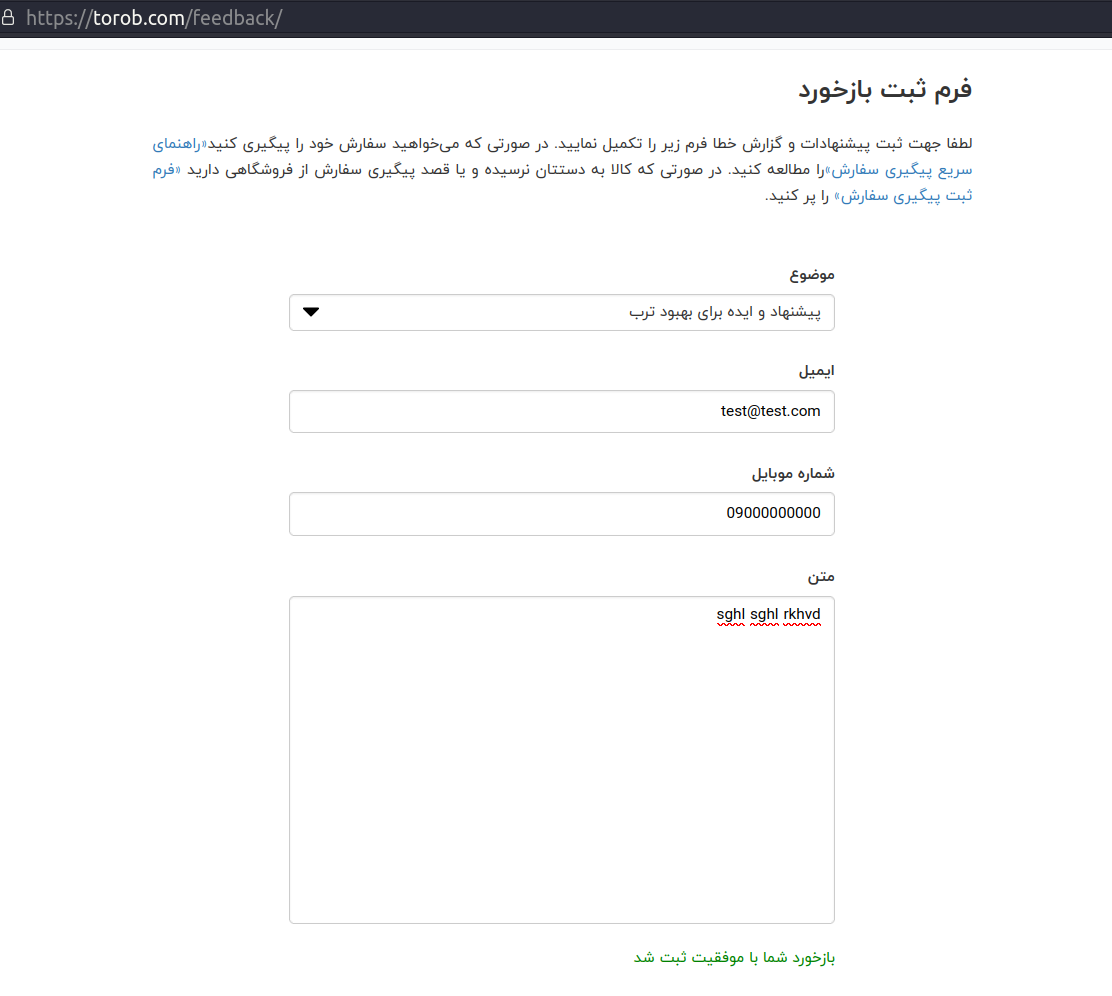
\includegraphics[width=0.7\linewidth]{figs/bug3}
	\caption[فرم بازخورد وبسایت ترب]{فرم بازخورد وبسایت ترب که در آن با وجود استفاده از یک شماره تماس غیرمعتبر بازخورد با موفقیت ثبت می‌شود.}
	\label{fig:bug3}
\end{figure}


\subsection*{مثال ۴}
\href{https://snappfood.ir/service/restaurant/city/Tehran/near?page=0&section=SERVICES&sort=max_rate&superType=1}{سامانه سفارش غذای آنلاین اسنپ‌فود.}
همان‌طور که در شکل \ref{fig:bug4} نیز قابل مشاهده است، در نمایش رستوران‌ها به ترتیب بالاترین امتیاز خطا وجود دارد. وجود چنین خطایی کاربر را به سایر فیلترها نیز بی‌اعتماد می‌کند و در نهایت از میزان رضایت آنها کاسته می‌شود.

\begin{figure}[H]
	\centering
	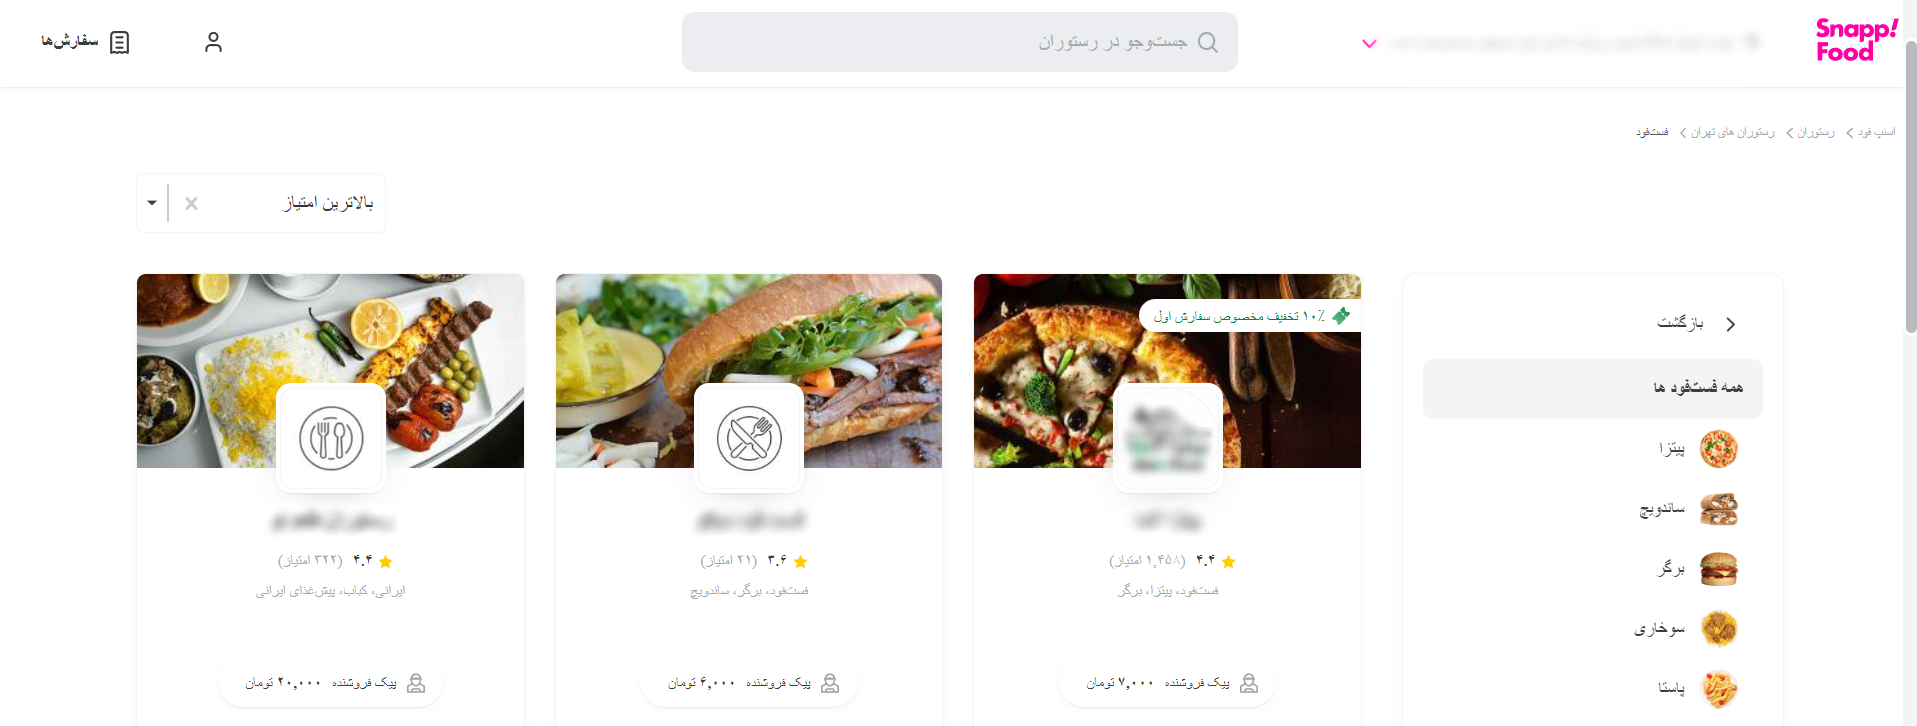
\includegraphics[width=0.7\linewidth]{figs/bug4.jpg}
	\caption{نمونه‌ای از ترتیب نامناسب در زمان نمایش رستوران‌ها بر اساس بالاترین امتیاز در سایت اسنپ‌فود.}
	\label{fig:bug4}
\end{figure}

\subsection*{مثال ۵}
\href{https://telegram.org/}{پیام‌رسان تلگرام}
این پیام‌رسان که با وجود محدودیت‌ها همچنان یکی از پرطرفدارترین نرم‌افزارهای ارتباطی‌است، خطای قابل توجهی در زمینه نشان دادن آخرین پیام ارسال شده دارد. در حالت عادی، در صفحه اصلی برنامه به ازای هر فرد/گروه، آخرین پیام ارسال شده در چند خط نمایش داده می‌شود. خطای این برنامه زمانی اتفاق می‌افتد که کاربری پیامی قبل از آخرین پیام خود را ویرایش می‌کند. در این صورت در صفحه اصلی برنامه به جای آخرین پیام، پیام ویرایش شده نشان داده می‌شود. عکس‌های مربوط به این خطا در شکل‌های \ref{fig:bug5} و \ref{fig:bug6} آورده شده‌‌اند.

\begin{figure}[H]
	\centering
	
\includegraphics[width=0.7\linewidth]{figs/bug5.jpg}
	\caption{صفحه پیام‌های یک کانال در تلگرام. با توجه به این شکل، کلمه \lr{"Hi"} باید از بیرون نمایش داده شود.}
	\label{fig:bug5}
\end{figure}

\begin{figure}[H]
	\centering
	
\includegraphics[width=0.7\linewidth]{figs/bug6.jpg}
	\caption{همان‌طور که در شکل مشخص است، کلمه ویرایش شده \lr{"Hihwl"} نشان داده شده است.}
	\label{fig:bug6}
\end{figure}

\subsection*{مراجع}

\begin{latin}
	\begingroup
	\renewcommand{\section}[2]{}%
	
\begin{thebibliography}{9}
	\bibitem{360logica}
	\textit{\href{https://www.360logica.com/blog/difference-between-defect-error-bug-failure-and-fault/
	}{360logica: difference between defect, error, bug, failure, and fault}}

	\bibitem{phoneregex}
	\textit{\href{https://www.datisnetwork.com/phone-number-regex.html}{phone number Regex}}

\end{thebibliography}
\endgroup
\end{latin}

}

